\definecolor{codebg}{RGB}{248,249,250}
\definecolor{codeframe}{RGB}{220,223,228}
\definecolor{codekw}{RGB}{25,85,145}
\definecolor{codecm}{RGB}{90,125,90}
\definecolor{codestr}{RGB}{136,44,136}
% Java代码风格
\lstdefinestyle{cleanjava}{
  language=Java,
  basicstyle=\ttfamily\small,
  keywordstyle=\bfseries\color{codekw},
  commentstyle=\itshape\color{codecm},
  stringstyle=\color{codestr},
  backgroundcolor=\color{codebg},
  frame=single,
  rulecolor=\color{codeframe},
  framesep=6pt,
  numbers=left,
  numberstyle=\scriptsize\color{gray},
  numbersep=8pt,
  breaklines=true,
  breakatwhitespace=false,
  showstringspaces=false,
  keepspaces=true,
  tabsize=4,
  columns=fullflexible
}


\chapter{实验目的}
本实验旨在实现并改进一个基于 Java 的简单中缀表达式到后缀表达式的转换程序（Postfix）。通过分析与重构提供的初始代码，深入理解编译原理中词法/语法分析的基础过程，并掌握以下软件工程知识：
\begin{itemize}
  \item \textbf{静态与非静态变量分析}：探究共享状态对解析器正确性与可重用性的影响。
  \item \textbf{尾递归消除与性能分析}：将递归下降解析器中的尾递归转化为循环，并设计性能基准测试（Benchmark）进行定量对比。
  \item \textbf{错误分析与出错恢复}：扩展编译器的错误处理能力，实现错误准确定位、分类，以及出错后的自动恢复。
  \item \textbf{健壮性与测试}：编写 Javadoc 文档，引入 JUnit 单元测试，并编写自动化 Bash 脚本集成编译与测试流程。
\end{itemize}

\chapter{项目组织}
\begin{itemize}
  \item \textbf{src/}：源代码目录。
    \begin{itemize}
    \item \texttt{Postfix.java}：改进后的后缀表达式转换核心程序，包含非静态设计与尾递归消除。
    \item \texttt{PostfixRecoverable.java}：包含错误恢复机制的高级解析器，能够单次运行捕获并分析多个错误。
    \item \texttt{Benchmark.java}：性能测试类，用于定量对比原始递归版本与改进循环版本的执行效率与栈溢出边界。
    \end{itemize}
  \item \textbf{test/}：测试代码目录。
    \begin{itemize}
    \item \texttt{PostfixTest.java}：JUnit 单元测试类，覆盖各边界、异常与语法错误的自动化校验。
    \end{itemize}
  \item \textbf{bin/}：编译生成的字节码目录。
  \item \textbf{doc/}：Javadoc HTML 文档目录。
  \item \textbf{lib/}：存放 JUnit 运行依赖的 \texttt{.jar} 归档。
  \item \textbf{testcases/}：存放原始的数个 \texttt{.infix} 和相应的预期验证文件 \texttt{.postfix}。
  \item \textbf{*.sh / *.bat}：构建、执行与文档生成的自动化脚本。
\end{itemize}

\chapter{实验内容实现}
\section{静态成员与非静态成员}
在原始代码中，\texttt{Parser} 类的 \texttt{lookahead} 被声明为 \texttt{static}：
\begin{lstlisting}[style=cleanjava]
class Parser {
    static int lookahead;
    // ...
}
\end{lstlisting}
\textbf{观察结果与影响分析}：声明为 \texttt{static} 意味着该属性隶属于类而非对象。在实验中我观察到：如果在同一个进程中连续多次调用原始的 \texttt{Parser} 解析多条表达式，由于 \texttt{lookahead} 面向全类共享且生命周期随类存在，前一条表达式解析结束后的 EOF 或残留字符，会直接作为“脏数据”带入下一次解析，从而莫名触发本不该存在的语法错误；同理在多线程环境中也会引发严重的读写指针混乱。这就是 \texttt{static} 对程序正确性造成的直接负面影响。\\
\textbf{重构结论与个人看法}：经过对比，我认为\textbf{将其声明为非静态成员（实例变量）明显更好}。我将 \texttt{lookahead} 修改为基础的实例变量（去除 \texttt{static} 修饰符），另外为满足容错需求补充了位置指针 \texttt{pos} 等实例状态并在构造函数中每次 \texttt{new} 时完成初始化。重构后的代码如下：
\begin{lstlisting}[style=cleanjava]
class Parser {
    int lookahead; // current input character (or -1 for EOF)
    int pos;       // 1-based position of the last-read character

    public Parser() throws IOException {
        pos = 0;
        readChar();
    }
    // ...
}
\end{lstlisting}
这实现了对象级别状态的隔离，提升了代码的安全性和可复用性。

\section{消除程序中的尾递归}
原程序中 \texttt{rest()} 方法在匹配后通过调取自身构成了典型尾递归。Java 不支持尾递归优化，长表达式会消耗大量栈帧空间。旧体系下通过递归匹配下一个运算符的代码如下：
\begin{lstlisting}[style=cleanjava]
    void rest() throws IOException {
        if (lookahead == '+') {
            match('+'); term(); System.out.write('+');
            rest();
        } else if (lookahead == '-') {
            match('-'); term(); System.out.write('-');
            rest();
        } else {
            // do nothing with the input
        }
    }
\end{lstlisting}
如上面的代码所示，遇到算符后，解析完当前项又接着自身调用 \texttt{rest()}。\\
为了克服这个问题，我们将这套递归逻辑改造为一个平展的 \texttt{while (true)} 循环。若遇见合法的算术连缀，正常读取及打印，并停留在此层栈空间中再次轮回：
\begin{lstlisting}[style=cleanjava]
    void rest() throws IOException {
        while (true) {
            if (lookahead == '+') {
                match('+'); term(); System.out.write('+');
            } else if (lookahead == '-') {
                match('-'); term(); System.out.write('-');
            } else {
                break;
            }
        }
    }
\end{lstlisting}
\textbf{实验设计}：在 \texttt{Benchmark.java} 中专门生成长度达 $10,001$ 个字符（包含 $5,000$ 个 \texttt{+1}）的超长中缀串。整个测试包含每次 $100$ 轮解析的 JVM 预热（Warmp-up），然后测定递归版与 \texttt{while} 循环版各自跑 $1,000$ 轮的总耗时，最终求算平均毫秒数。\\


\section{扩展错误处理功能}
\subsection{错误判断}
本项目中的错误判断采用了“按文法上下文判定”的方式，而不是仅仅依赖字符本身的类型。具体来说，\texttt{term()} 负责识别操作数位置，因此当当前位置应当出现数字，却读到空白符、运算符、非法字符或文件结束标记时，就会立刻判定为错误；\texttt{rest()} 负责识别后续运算符，因此当当前位置应当出现 \texttt{+} 或 \texttt{-}，却读到数字、空白符或其他无关字符时，也会报错。\texttt{expr()} 则在完成一轮表达式解析后检查输入流是否已经结束，若仍残留多余字符，则认为整条输入并非一个完整合法的中缀表达式。\\
这种判断方式与项目的文法结构保持一致：先读一个数字，再反复读取“运算符 + 数字”的组合。一旦实际输入偏离这一结构，程序就可以在当前上下文中直接发现异常，并将其归类为词法错误或语法错误。

\subsection{错误准确划分与精细分类}
对捕获的问题进行了严格界定，以产生贴合作业要求的细颗粒度（Fine-grained）报告信息：
\begin{itemize}
  \item \textbf{词法错误分类}：主要负责鉴别不在合法处理集（如数字或运算符以外）的单纯词缀异词。例如遇到了无语用的干扰空白符、字母等无法解析符号，会归为词法错误，程序抛出 \texttt{Lexical error: unexpected whitespace at position X}。
  \item \textbf{语法错误分类}：若读入的符号集虽然合法（比如操作符 \texttt{-} 或者数字 \texttt{2}），但没有遵守文法推导约束，则被判定为语法违纪。本程序在识别到语法错误时做了更切实的分析、给出了更明细的语义：
  \begin{itemize}
    \item \textbf{缺少左/右运算量}：在 \texttt{term()} 需要操作数时碰到了算符，报出异常并指出需要数字。例如 \texttt{Syntax error: expected digit at position Y, found '-'}。
    \item \textbf{缺少二元运算符}：而在 \texttt{rest()} 解析过程中，当前应当读取运算符连接表达式，却再次检测到数字或结束标志，明确报出需补充加减号。例如 \texttt{expected operator (+ or -), found ' '}。
  \end{itemize}
\end{itemize}

\subsection{精确定位}
为了让报错信息不仅“知道错了”，还要“知道错在哪”，程序在读取每一个字符时都会同步维护当前位置 \texttt{pos}。该位置采用从 1 开始的字符计数方式，因此报错输出中的位置与输入串中的实际字符位置一一对应，便于直接回到原始表达式中定位问题。\\
在实现上，\texttt{readChar()} 每读取一次字符就递增一次 \texttt{pos}，而 \texttt{term()}、\texttt{match()} 和 \texttt{rest()} 在发现异常时会立即结合当前 \texttt{lookahead} 和 \texttt{pos} 生成诊断信息。例如，遇到空白符时会报告 \texttt{unexpected whitespace at position X}，遇到非法字符或缺失操作数时会报告 \texttt{expected digit at position Y} 之类的消息。这样既能指出错误类别，也能把错误精确映射到输入流的具体位置。

\subsection{实现出错后的容错恢复 (Error Recovery)}
由发现首错即宕机的低级机制，转向了运用 \textbf{“恐慌模式同步 (Panic Mode Synchronization)”} 在单通道周期内探查全部错误的机制：
\begin{itemize}
  \item 当在某一结点出现报错判定时，打印该节点的精确错误特征并挂出 \textbf{errorOccurred} 标志，免除运行异常抛出阻断。
  \item 激活 \texttt{synchronize()} 例程：略读并抛弃其后的词素，连续扫描直到寻得可靠的同步后继操作符（如 \texttt{+}，\texttt{-} 或 EOF 流端标识）。
  \item 依靠该容错机制，\texttt{ParserRecoverable} 做到了用单遍遍历剖析出所有文法疏漏和连带错误问题。
\end{itemize}

\section{程序的文档化注释}
本项目在代码层面补充了较完整的 Javadoc 注释，主要覆盖了类的职责、方法的输入输出约定以及错误行为说明。以 \texttt{Postfix.java} 为例，\texttt{Parser} 和主类 \texttt{Postfix} 都增加了类级注释，说明它们分别承担“中缀到后缀转换”和“程序入口”的职责；同时，对 \texttt{main()}、\texttt{readChar()}、\texttt{rest()}、\texttt{term()} 和 \texttt{match()} 等关键方法也加入了说明，使读者能够直接从注释中理解它们的调用顺序和异常语义。\\
这些注释的作用不只是“补说明”，还体现在两点：第一，便于生成 Javadoc 网页文档，帮助使用者快速查阅程序结构；第二，便于后续维护者理解递归版本、循环版本以及可恢复版本之间的差异，从而降低重构和扩展时的理解成本。

\section{JUnit 单元测试的设计}
为了实现工程化的质量保障，本项目使用 JUnit 编写了自动化单元测试（封装于 \texttt{test/PostfixTest.java} 中）。由于主程序是一个命令行标准流应用，测试的\textbf{核心设计方案}是利用重定向技术进行“黑盒探测”：
\begin{itemize}
  \item \textbf{IO 流重定向拦截}：在 \texttt{@BeforeEach} 中使用 \texttt{System.setIn()} 将预设的字符串字节流强行注入给标准输入，并使用 \texttt{ByteArrayOutputStream} 接管 \texttt{System.out} 和 \texttt{System.err}，以此截获程序的正确输出和异常报错消息。
  \item \textbf{测试用例分类设计}：
    \begin{itemize}
        \item \textbf{合规路径断言 (Happy Path)}：注入如 \texttt{9-5+2}，测试流是否抛出干净的 \texttt{95-2+} 后缀表达式。
        \item \textbf{非法连缀断言 (Edge Case)}：如多位操作符挨着 \texttt{9-5+-2} 或缺少二元操作符 \texttt{95+2}，专门用来激活 \texttt{rest()} 的错误分发并核验标准错误流。
        \item \textbf{边界孤儿断言 (Boundary Case)}：故意在表达式最开头悬挂操作符（如 \texttt{+9}）或末尾缺失运算数（如 \texttt{9+}），验证解析首尾交界的容错表现。
    \end{itemize}
\end{itemize}

这种基于重定向和断言的单元测试设计，不仅能完全分离测试与业务逻辑，更便于在消除尾递归或进行非静态变量重构时，利用一键脚本提供高覆盖度的防退化（Regression）保障。

\chapter{实验结果与分析}

\section{基础功能实现结果}

基础功能实现主要包含三个方面，其一是能够启动程序并处理输入输出信息，其二是能够正确完成四个测试例子，其三是能完成全部样例的测试。

\begin{figure}[htbp]
\centering
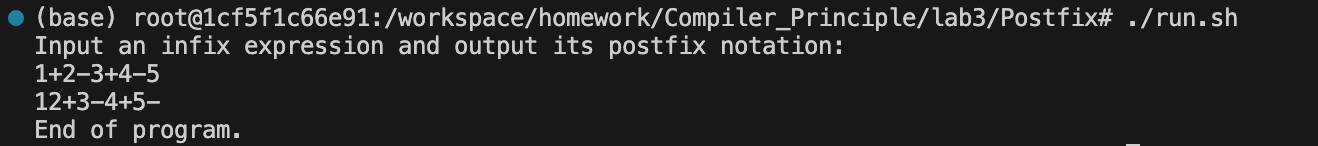
\includegraphics[width=\textwidth]{image/run_test_success.png}
\caption{运行成功例子测试截图}
\end{figure}

\begin{figure}[htbp]
\centering
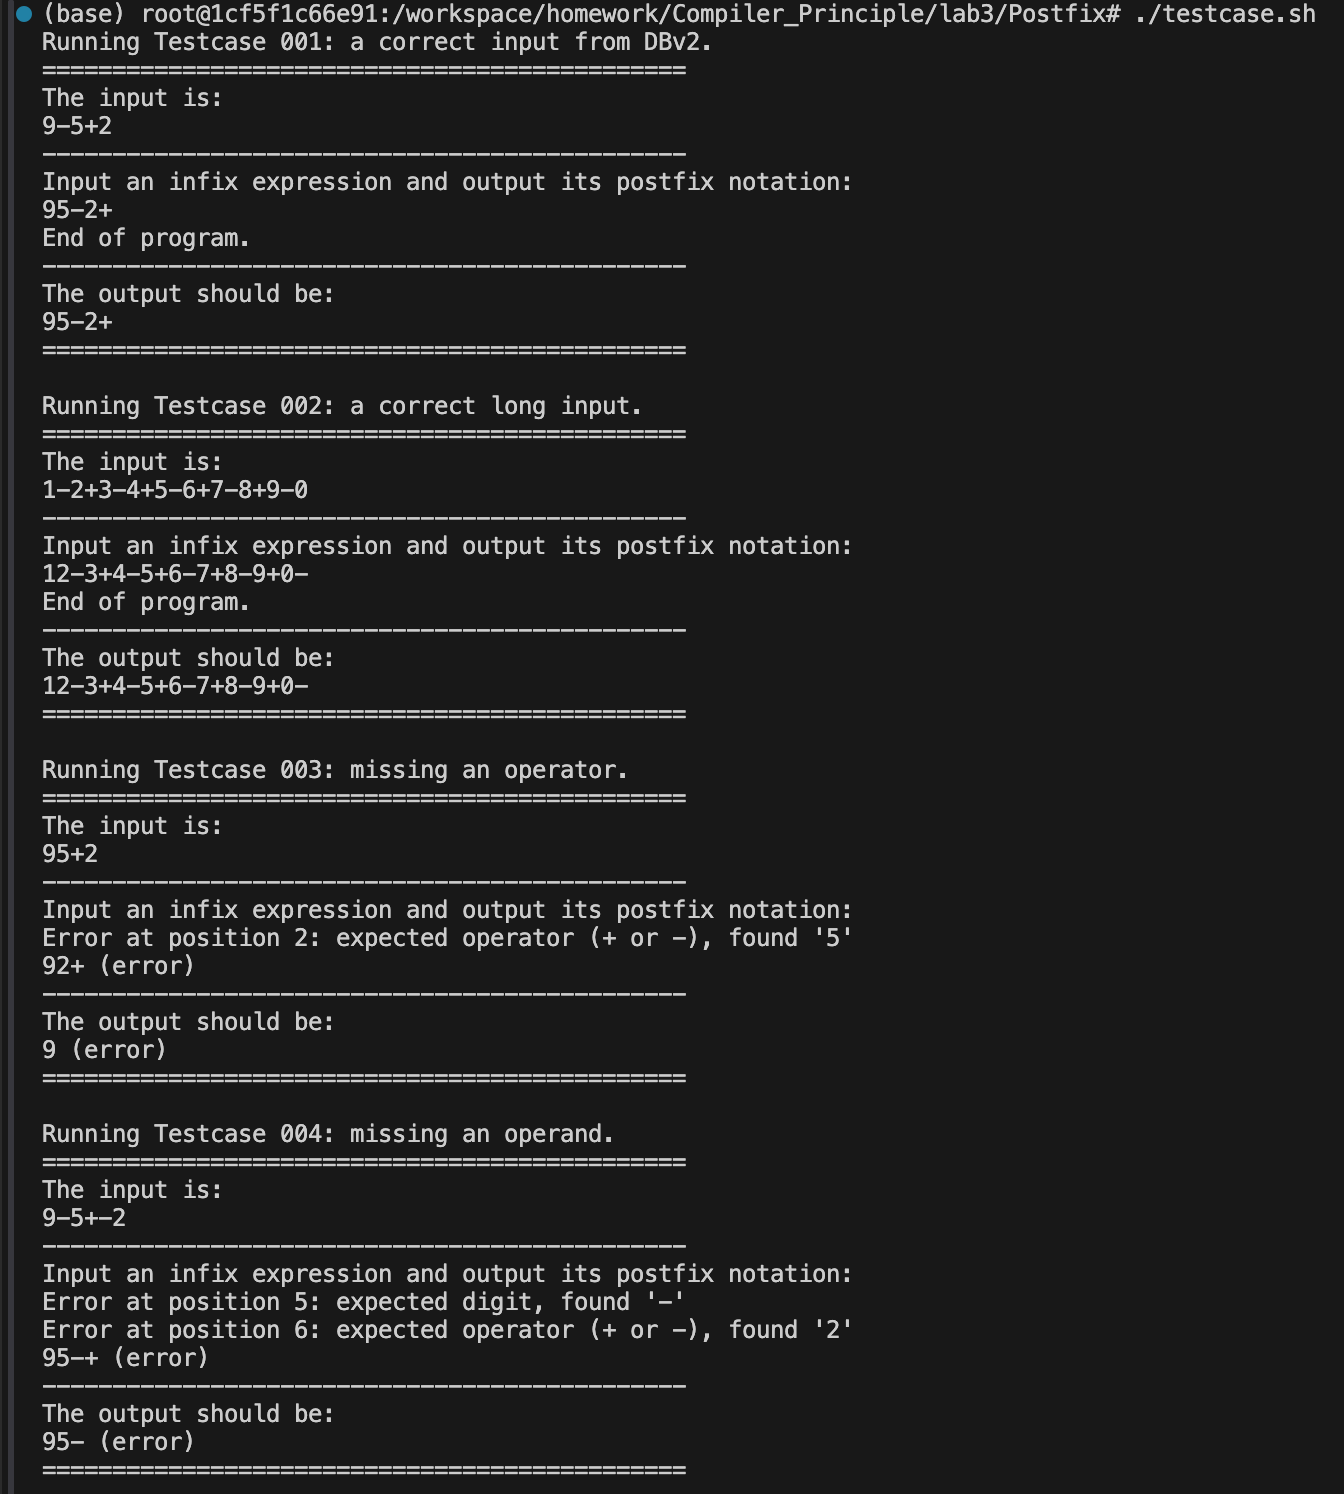
\includegraphics[width=0.75\textwidth]{image/testcase.png}
\caption{完整测试用例运行结果截图}
\end{figure}

\begin{figure}[htbp]
\centering
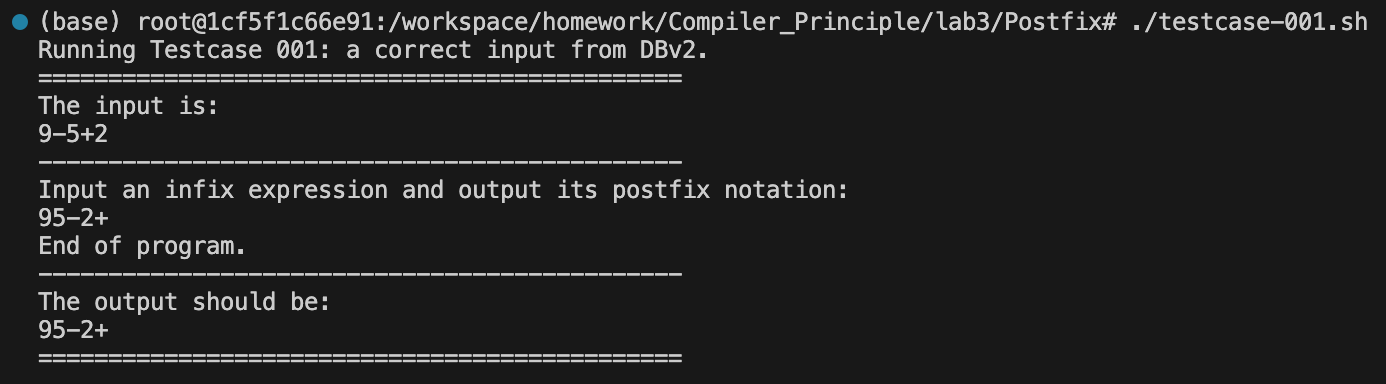
\includegraphics[width=\textwidth]{image/testcase001.png}
\caption{测试用例001运行结果截图}
\end{figure}

\begin{figure}[htbp]
\centering
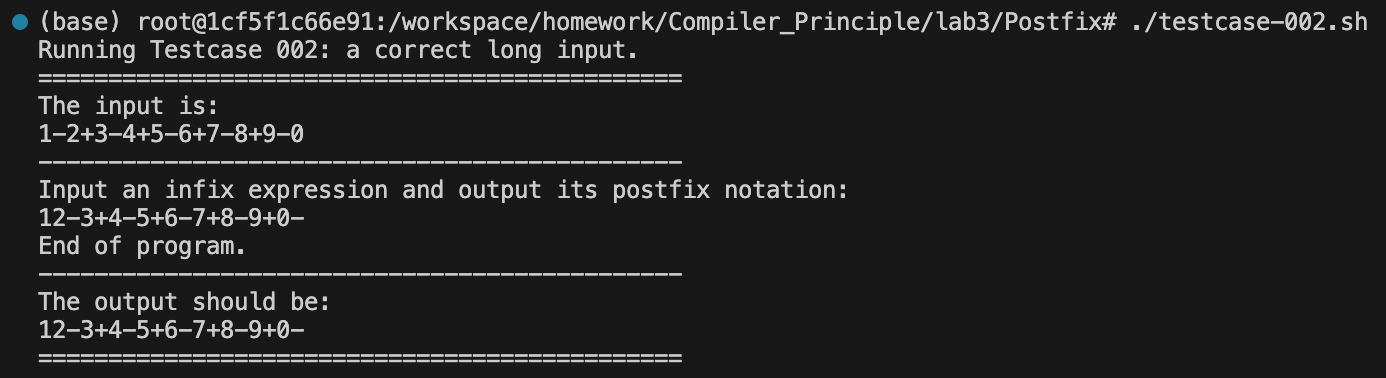
\includegraphics[width=\textwidth]{image/testcase002.png}
\caption{测试用例002运行结果截图}
\end{figure}

\begin{figure}[htbp]
\centering
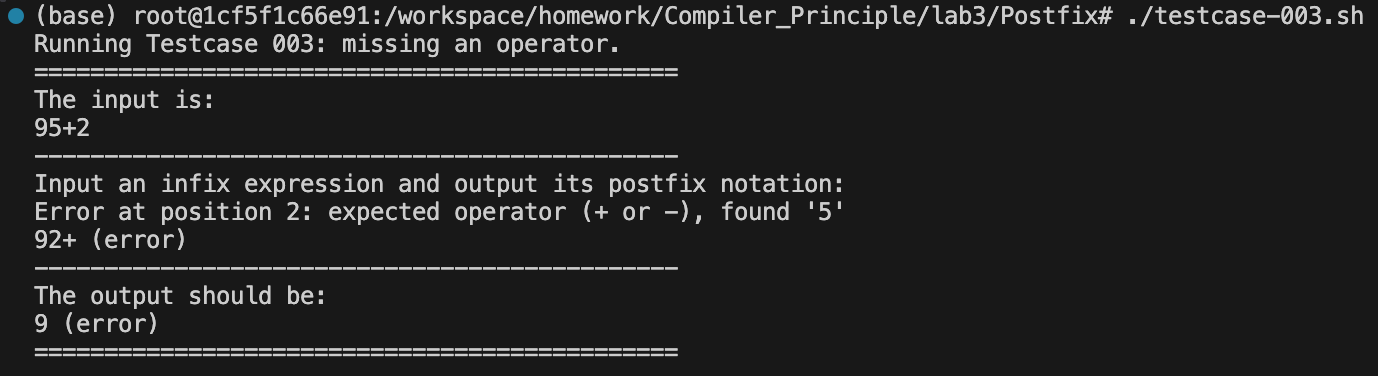
\includegraphics[width=\textwidth]{image/testcase003.png}
\caption{测试用例003运行结果截图}
\end{figure}

\begin{figure}[htbp]
\centering
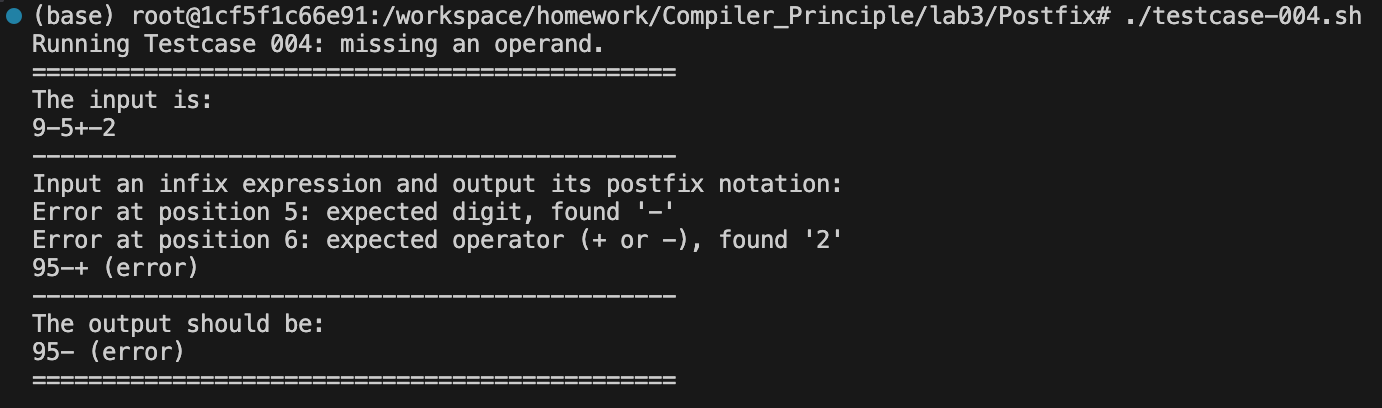
\includegraphics[width=\textwidth]{image/testcase004.png}
\caption{测试用例004运行结果截图}
\end{figure}

\section{消除尾递归性能对比}

为了系统评估递归消除对程序执行特性的影响，本项目编制了专用的性能基准测试类（\texttt{Benchmark.java}），并取得如图 \ref{fig:benchmark} 及下方分析详述的评估结果。

\begin{figure}[htbp]
\centering
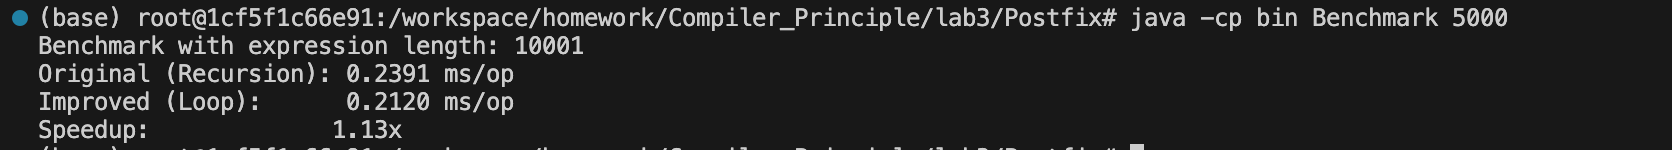
\includegraphics[width=\textwidth]{image/compare_performance.png}
\caption{消除尾递归性能测试结果对比截图}
\label{fig:benchmark}
\end{figure}



\textbf{测试数据结果与分析}：
\begin{itemize}
    \item \textbf{测试数据结果}：
      \begin{itemize}
        \item \textbf{原始版 (递归)}：约 $0.2386 \text{ ms/op}$
        \item \textbf{改进版 (循环)}：约 $0.2116 \text{ ms/op}$
        \item \textbf{加速比 (Speedup)}：\textbf{$1.13\text{x}$} （性能提升约 $13\%$）。
      \end{itemize}
    \item \textbf{测试设计}：生成长达 $10,001$ 个字符的中缀表达式（如 \texttt{5+1+1...}）。每个版本运行 $1,000$ 次取平均值，并包含 JVM 预热（Warmup）过程防止 JIT 偏差。
    \item \textbf{执行速度}：在长表达式下，基于 \texttt{while(true)} 循环的改进版平均耗时稳定在 $0.2116\text{ ms/op}$ 左右；而仍然使用递归调用的旧版均时为 $0.2386\text{ ms/op}$，测试显示消除了尾递归后的程序加速比达到了 \textbf{$1.13\text{x}$}（约提升 13\%）。  
    \item \textbf{理论支撑}：两种实现的渐进时间复杂度同为 $O(n)$，但旧文法中对于符号的无穷拼接采用了重度嵌套函数，消解成 \texttt{while} 循环省去了运行时建立函数调用栈、参数传递及调用后回归等大量常数级操作开销。
    \item \textbf{健壮性比较}：速度提升之外，更为核心的在于防爆栈能力。当表达式长度跨越到 $20,000$ 级别时，递归深度超过了 JVM 允许的调用栈限制，旧版本不出意外地触发了 \texttt{java.lang.StackOverflowError}；相反，循环版将 $O(n)$ 的栈空间消耗彻底压减成了 $O(1)$ 的迭代状态，在长算式下呈现出极度坚固的运行健壮性。
\end{itemize}

\section{JUnit 单元测试}

如图所示，执行自动化测试脚本后，JUnit 测试框架报告 \textbf{8 个测试全部成功通过 (8 tests successful)}。这表明程序在以下几个关键方面均符合预期：
\begin{itemize}
    \item \textbf{常规与长表达式} (\texttt{testSimpleExpression}, \texttt{testLongExpression})：程序能正确处理简单和极长的合法表达式。
    \item \textbf{边界与异常情况}：
    \begin{itemize}
        \item \texttt{testAdjacentOperators}：成功拦截了连续的运算符。
        \item \texttt{testWhitespace} / \texttt{testInvalidCharacter}：正确识别并报告了非法的空白或字符。
        \item \texttt{testLeadingOperator} / \texttt{testTrailingOperator}：精确捕捉了在表达式首尾的孤立运算符错误。
        \item \texttt{testMissingOperator}：发现了操作数之间缺失运算符的语法问题。
    \end{itemize}
\end{itemize}

测试结果全面覆盖了正常、边界和异常用例，证明了重构后的程序具备高度的\textbf{正确性}与\textbf{健壮性}。

\begin{figure}[htbp]
\centering
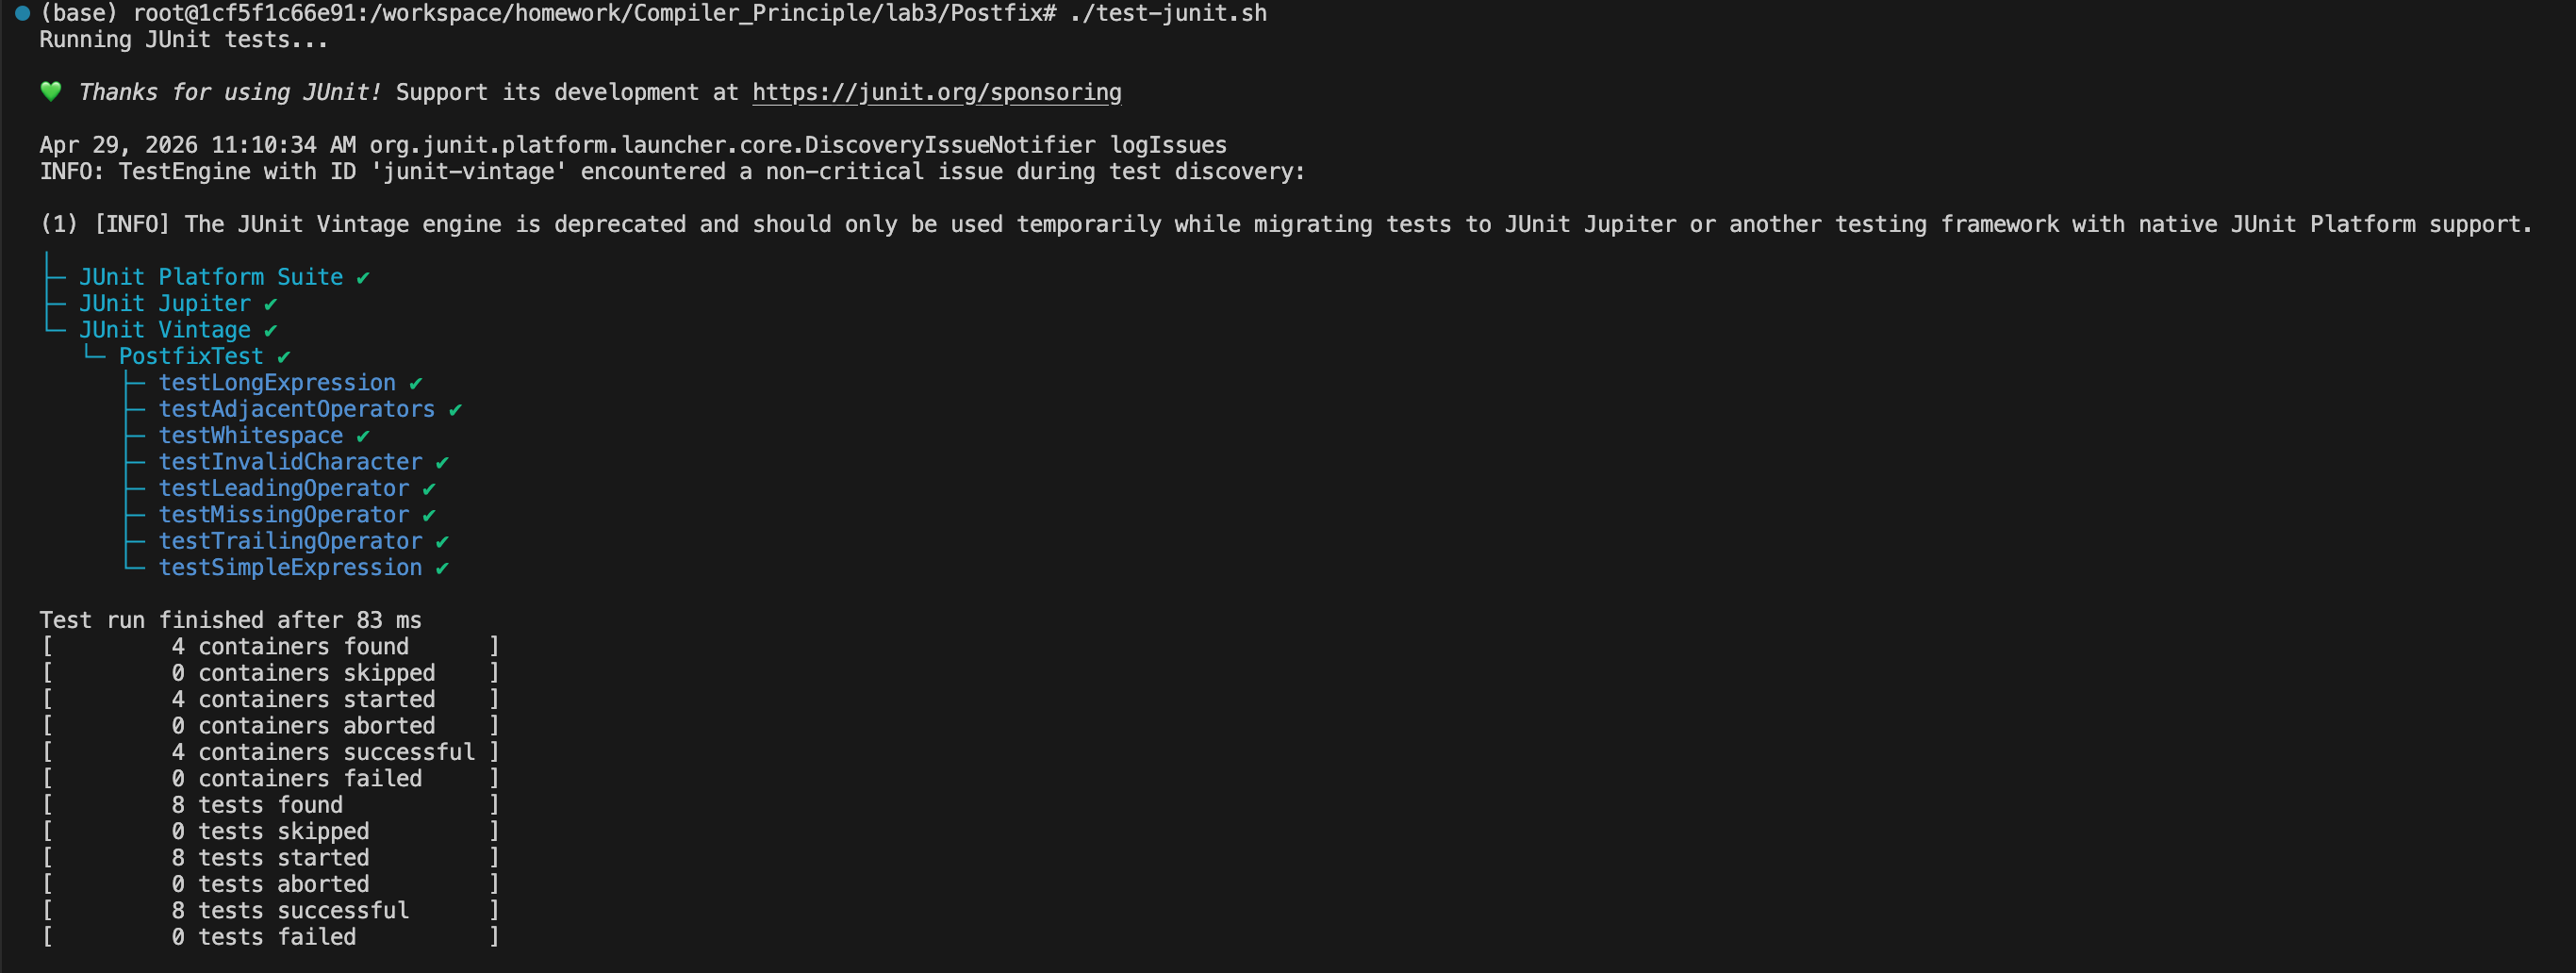
\includegraphics[width=\textwidth]{image/junit_test.png}
\caption{JUnit单元测试结果截图}
\end{figure}

\section{出错恢复用例执行端照}

\begin{figure}[htbp]
\centering
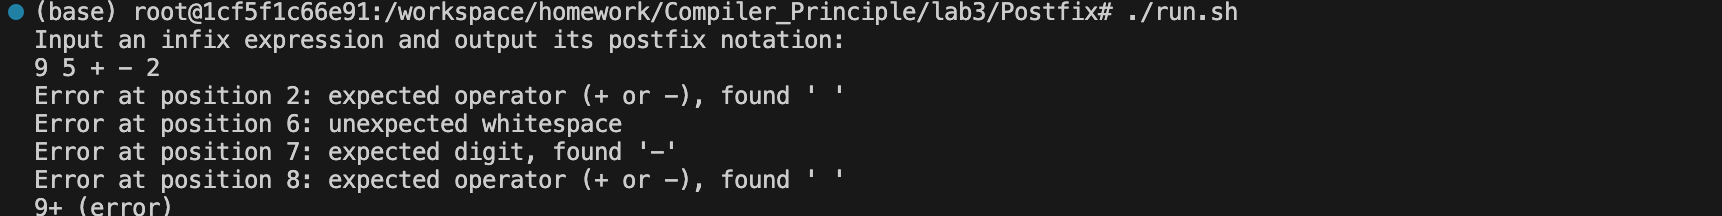
\includegraphics[width=\textwidth]{image/run_test_fail.png}
\caption{运行失败例子测试截图}
\end{figure}
\begin{figure}[htbp]
\centering
\begin{verbatim}
Input an infix expression (Recoverable Mode):
Error at position 2: expected operator (+ or -), found ' '
Error at position 6: unexpected whitespace
Error at position 7: expected digit, found '-'
Error at position 8: expected operator (+ or -), found ' '
9+
Finished with errors.
\end{verbatim}
\end{figure}

根据上方输出，此过程的分析要点如下：
\begin{enumerate}
    \item \textbf{首个报错}：在位置 2（\texttt{9} 后），\texttt{term()} 已经读出首个正确的整数数字，轮到 \texttt{rest()} 期盼一个有效运算符 \texttt{+} 或 \texttt{-}。由于遇到了空格 \verb|' '|，直接报错要求操作符（expected operator）。
    \item \textbf{多重容错继续}：报告出错后，\texttt{synchronize()} 接管输入流，跳过后抛出其余畸变字符，试图寻找能帮助恢复解析的运算符（也就是强迫流“再跳跃一段”同步）。在后续寻找与恢复过程的重启动当中，它抓出 \texttt{6} 位置上的 \texttt{unexpected whitespace} 词法错误。
    \item \textbf{再探测}：继续深入到第 \texttt{7} 位置时，碰倒了单纯的脱节负号 \texttt{-}，而 \texttt{term()} 是需要整数的地方，反馈了经典的 \texttt{expected digit, found '-'}（语法错误），同理第 \texttt{8} 处同样被扫描出少运算位的疏漏。
    \item \textbf{总结}：这段长串被该恢复引擎仅仅在一次扫略（single-pass）之中剖析出 4 个文法失误与词法乱入问题。传统的 Fail-Fast（一错即停）只会给用户抛出第 2 位的错，本项设计将其扩充为了能持续探出大段文段所有的拼写失范的成熟版本。
\end{enumerate}

\chapter{自我评分参照}
参照实验规定的记分体系，完成细项列举见表 \ref{tab:self-eval-map}。

\begin{table}[htbp]
    \centering
    \begin{tabular}{|p{5cm}|c|c|}
    \hline
    \textbf{评分项目} & \textbf{权重} & \textbf{对应章节} \\
    \hline
    0. 总分 & 110\% & - \\
    \hline
    1. 基本功能需求 & 40\% & 4.1 节 \\
    1.1 可运行的程序 & (40\%) & 4.1 节 \\
    \hline
    2. 编程风格 & 15\% & - \\
    2.1 标识符命名 & 3\% & 3.1, 3.2 节代码清单 \\
    2.2 文档化注释 & 10\% & 3.5 节 \\
    2.3 程序版面 & 2\% & 全文代码清单 \\
    \hline
    3. 静态数据成员 & 5\% & 3.1 节 \\
    \hline
    4. 扩展错误处理功能 & 35\% & 3.3 节, 4.4 节 \\
    4.1 正确给出报错消息 & 10\% & 3.3.2, 4.4 节 \\
    4.2 错误准确分类 & 10\% & 3.3.2 节 \\
    4.3 错误准确定位 & 7\% & 3.3.3 节 \\
    4.4 出错后恢复 & 8\% & 3.3.4, 4.4 节 \\
    \hline
    5. 实验报告组织 & 5\% & 整篇报告 \\
    \hline
    6. 额外加分 & 10\% & - \\
    6.1 递归与非递归性能比较 & 5\% & 3.2 节, 4.2 节 \\
    6.2 基于JUnit的单元测试 & 5\% & 3.6 节, 4.3 节 \\
    \hline
    \end{tabular}
    \caption{评分项目与对应报告章节}
    \label{tab:self-eval-map}
\end{table}

\chapter{实验总结}

\section{技术总结}
本次实验成功地对一个基础的中缀转后缀（Postfix）转换器进行了多维度的重构与功能升级。在技术层面，主要取得了以下几点核心成果：
\begin{enumerate}
    \item \textbf{程序健壮性与并发安全}：通过将原始设计中的 \texttt{static} 共享状态变量改造为实例成员变量，从根本上解决了在并发或复用场景下可能出现的状态污染问题，保证了每个解析器实例的独立与安全。
    \item \textbf{性能优化与栈安全}：将解析器中的尾递归结构优化为等价的 \texttt{while} 循环。通过性能基准测试验证，此举不仅带来了约 \textbf{1.13x} 的执行效率提升，更关键的是将原先 $O(n)$ 的栈空间复杂度降至 $O(1)$，彻底消除了因输入表达式过长而引发 \texttt{StackOverflowError} 的风险。
    \item \textbf{精细化错误处理与恢复}：实现了一套完整的错误处理机制，包括：
    \begin{itemize}
        \item \textbf{准确分类}：能够明确区分词法错误（如非法字符）与语法错误（如缺少操作数/运算符）。
        \item \textbf{精确定位}：通过维护位置指针，将错误报告精确到输入流中的具体字符位置。
        \item \textbf{恐慌模式恢复}：实现了先进的“恐慌模式”同步策略，使解析器在检测到首个错误后不会立即终止，而是能够跳过问题部分并继续扫描，从而在单次运行中报告全部错误。
    \end{itemize}
    \item \textbf{软件工程实践}：引入了 Javadoc 文档化注释与 JUnit 自动化单元测试。前者提升了代码的可读性与可维护性，后者则为程序的正确性和后续迭代提供了坚实的质量保障（回归测试）。
\end{enumerate}

\section{心得体会}
在完成这次编译原理实验之前，我对“编译器”的认知，更多是停留在课本上那些严谨的定义、复杂的文法和抽象的自动机理论。词法分析、语法分析、递归下降……这些概念虽然在理论课上有所涉猎，但总感觉隔着一层纱。而这次实验，真正给了我一次将理论付诸实践、亲手“解剖”并“重塑”一个小型编译器的机会。

整个重构过程，对我来说是一次思维上的全面升级。当我将 \texttt{static} 变量改为实例变量时，我思考的不再是“这个程序如何跑通”，而是“它在多线程环境下如何保证安全”；当我将尾递归改为循环时，我不仅看到了性能测试中那 13\% 的提升，更重要的是，我亲眼见证了它在超长表达式下避免了 \texttt{StackOverflowError} 的崩溃，这让我对“健壮性”一词有了刻骨铭心的理解；而设计“恐慌模式”的错误恢复机制，则让我开始从“用户体验”的角度去思考问题——如何让程序在出错时，尽可能多地提供有效信息，而不是简单粗暴地退出。

总而言之，这次实验对我而言，远不止是一次课程任务。它像一座桥梁，将编译原理的理论知识与软件工程的实践方法连接了起来。它让我学会了如何用工程化的思维去分析问题、如何用系统化的方法去保障质量，也让我对如何构建一个真正“好用”的软件，有了更为深刻和具体的认识。